\documentclass[twoside]{book}

% Packages required by doxygen
\usepackage{fixltx2e}
\usepackage{calc}
\usepackage{doxygen}
\usepackage[export]{adjustbox} % also loads graphicx
\usepackage{graphicx}
\usepackage[utf8]{inputenc}
\usepackage{makeidx}
\usepackage{multicol}
\usepackage{multirow}
\PassOptionsToPackage{warn}{textcomp}
\usepackage{textcomp}
\usepackage[nointegrals]{wasysym}
\usepackage[table]{xcolor}

% Font selection
\usepackage[T1]{fontenc}
\usepackage[scaled=.90]{helvet}
\usepackage{courier}
\usepackage{amssymb}
\usepackage{sectsty}
\renewcommand{\familydefault}{\sfdefault}
\allsectionsfont{%
  \fontseries{bc}\selectfont%
  \color{darkgray}%
}
\renewcommand{\DoxyLabelFont}{%
  \fontseries{bc}\selectfont%
  \color{darkgray}%
}
\newcommand{\+}{\discretionary{\mbox{\scriptsize$\hookleftarrow$}}{}{}}

% Page & text layout
\usepackage{geometry}
\geometry{%
  a4paper,%
  top=2.5cm,%
  bottom=2.5cm,%
  left=2.5cm,%
  right=2.5cm%
}
\tolerance=750
\hfuzz=15pt
\hbadness=750
\setlength{\emergencystretch}{15pt}
\setlength{\parindent}{0cm}
\setlength{\parskip}{3ex plus 2ex minus 2ex}
\makeatletter
\renewcommand{\paragraph}{%
  \@startsection{paragraph}{4}{0ex}{-1.0ex}{1.0ex}{%
    \normalfont\normalsize\bfseries\SS@parafont%
  }%
}
\renewcommand{\subparagraph}{%
  \@startsection{subparagraph}{5}{0ex}{-1.0ex}{1.0ex}{%
    \normalfont\normalsize\bfseries\SS@subparafont%
  }%
}
\makeatother

% Headers & footers
\usepackage{fancyhdr}
\pagestyle{fancyplain}
\fancyhead[LE]{\fancyplain{}{\bfseries\thepage}}
\fancyhead[CE]{\fancyplain{}{}}
\fancyhead[RE]{\fancyplain{}{\bfseries\leftmark}}
\fancyhead[LO]{\fancyplain{}{\bfseries\rightmark}}
\fancyhead[CO]{\fancyplain{}{}}
\fancyhead[RO]{\fancyplain{}{\bfseries\thepage}}
\fancyfoot[LE]{\fancyplain{}{}}
\fancyfoot[CE]{\fancyplain{}{}}
\fancyfoot[RE]{\fancyplain{}{\bfseries\scriptsize Generated by Doxygen }}
\fancyfoot[LO]{\fancyplain{}{\bfseries\scriptsize Generated by Doxygen }}
\fancyfoot[CO]{\fancyplain{}{}}
\fancyfoot[RO]{\fancyplain{}{}}
\renewcommand{\footrulewidth}{0.4pt}
\renewcommand{\chaptermark}[1]{%
  \markboth{#1}{}%
}
\renewcommand{\sectionmark}[1]{%
  \markright{\thesection\ #1}%
}

% Indices & bibliography
\usepackage{natbib}
\usepackage[titles]{tocloft}
\setcounter{tocdepth}{3}
\setcounter{secnumdepth}{5}
\makeindex

% Hyperlinks (required, but should be loaded last)
\usepackage{ifpdf}
\ifpdf
  \usepackage[pdftex,pagebackref=true]{hyperref}
\else
  \usepackage[ps2pdf,pagebackref=true]{hyperref}
\fi
\hypersetup{%
  colorlinks=true,%
  linkcolor=blue,%
  citecolor=blue,%
  unicode%
}

% Custom commands
\newcommand{\clearemptydoublepage}{%
  \newpage{\pagestyle{empty}\cleardoublepage}%
}

\usepackage{caption}
\captionsetup{labelsep=space,justification=centering,font={bf},singlelinecheck=off,skip=4pt,position=top}

%===== C O N T E N T S =====

\begin{document}

% Titlepage & ToC
\hypersetup{pageanchor=false,
             bookmarksnumbered=true,
             pdfencoding=unicode
            }
\pagenumbering{alph}
\begin{titlepage}
\vspace*{7cm}
\begin{center}%
{\Large My Project }\\
\vspace*{1cm}
{\large Generated by Doxygen 1.8.14}\\
\end{center}
\end{titlepage}
\clearemptydoublepage
\pagenumbering{roman}
\tableofcontents
\clearemptydoublepage
\pagenumbering{arabic}
\hypersetup{pageanchor=true}

%--- Begin generated contents ---
\chapter{Class Index}
\section{Class List}
Here are the classes, structs, unions and interfaces with brief descriptions\+:\begin{DoxyCompactList}
\item\contentsline{section}{\mbox{\hyperlink{structdroga}{droga}} }{\pageref{structdroga}}{}
\item\contentsline{section}{\mbox{\hyperlink{structmiasto}{miasto}} }{\pageref{structmiasto}}{}
\item\contentsline{section}{\mbox{\hyperlink{structwynik}{wynik}} }{\pageref{structwynik}}{}
\end{DoxyCompactList}

\chapter{Class Documentation}
\hypertarget{structdroga}{}\section{droga Struct Reference}
\label{structdroga}\index{droga@{droga}}


{\ttfamily \#include $<$struktury.\+h$>$}



Collaboration diagram for droga\+:
\nopagebreak
\begin{figure}[H]
\begin{center}
\leavevmode
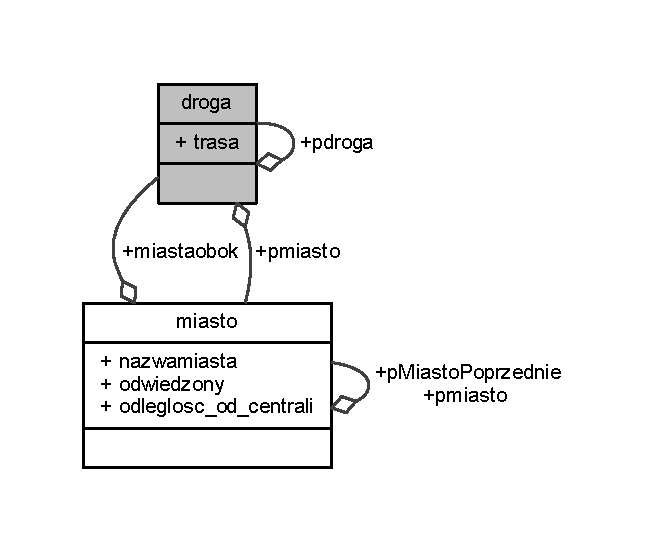
\includegraphics[width=310pt]{structdroga__coll__graph}
\end{center}
\end{figure}
\subsection*{Public Attributes}
\begin{DoxyCompactItemize}
\item 
int \mbox{\hyperlink{structdroga_a4788083344d3da2783792f80b35ab524}{trasa}}
\item 
\mbox{\hyperlink{structdroga}{droga}} $\ast$ \mbox{\hyperlink{structdroga_a7ed57ce3de3b4184ba7f7c805964626f}{pdroga}}
\item 
\mbox{\hyperlink{structmiasto}{miasto}} $\ast$ \mbox{\hyperlink{structdroga_a9c782b9f5281ee0f4cb4581a364b4471}{pmiasto}}
\end{DoxyCompactItemize}


\subsection{Detailed Description}
Struktura droga 
\begin{DoxyParams}{Parameters}
{\em trasa} & odleglosc miedzy miastami \\
\hline
{\em pdroga} & wskaznik na nastepna droge \\
\hline
{\em pmiasto} & wskaznik na odpowiednie miasto \\
\hline
\end{DoxyParams}


\subsection{Member Data Documentation}
\mbox{\Hypertarget{structdroga_a7ed57ce3de3b4184ba7f7c805964626f}\label{structdroga_a7ed57ce3de3b4184ba7f7c805964626f}} 
\index{droga@{droga}!pdroga@{pdroga}}
\index{pdroga@{pdroga}!droga@{droga}}
\subsubsection{\texorpdfstring{pdroga}{pdroga}}
{\footnotesize\ttfamily \mbox{\hyperlink{structdroga}{droga}}$\ast$ droga\+::pdroga}

\mbox{\Hypertarget{structdroga_a9c782b9f5281ee0f4cb4581a364b4471}\label{structdroga_a9c782b9f5281ee0f4cb4581a364b4471}} 
\index{droga@{droga}!pmiasto@{pmiasto}}
\index{pmiasto@{pmiasto}!droga@{droga}}
\subsubsection{\texorpdfstring{pmiasto}{pmiasto}}
{\footnotesize\ttfamily \mbox{\hyperlink{structmiasto}{miasto}}$\ast$ droga\+::pmiasto}

\mbox{\Hypertarget{structdroga_a4788083344d3da2783792f80b35ab524}\label{structdroga_a4788083344d3da2783792f80b35ab524}} 
\index{droga@{droga}!trasa@{trasa}}
\index{trasa@{trasa}!droga@{droga}}
\subsubsection{\texorpdfstring{trasa}{trasa}}
{\footnotesize\ttfamily int droga\+::trasa}



The documentation for this struct was generated from the following file\+:\begin{DoxyCompactItemize}
\item 
\mbox{\hyperlink{struktury_8h}{struktury.\+h}}\end{DoxyCompactItemize}

\hypertarget{structmiasto}{}\section{miasto Struct Reference}
\label{structmiasto}\index{miasto@{miasto}}


{\ttfamily \#include $<$struktury.\+h$>$}



Collaboration diagram for miasto\+:
% FIG 0
\subsection*{Public Attributes}
\begin{DoxyCompactItemize}
\item 
std\+::string \mbox{\hyperlink{structmiasto_a75a023beb08b889860c2068ffd47318e}{nazwamiasta}}
\item 
\mbox{\hyperlink{structmiasto}{miasto}} $\ast$ \mbox{\hyperlink{structmiasto_a9cd7b8d4e3e00ba833d3149b76a918f9}{pmiasto}}
\item 
\mbox{\hyperlink{structdroga}{droga}} $\ast$ \mbox{\hyperlink{structmiasto_af69437beea5c134e233947df273a48a4}{miastaobok}}
\item 
bool \mbox{\hyperlink{structmiasto_a7a2028174edb36e184c06d084d02ef27}{odwiedzony}}
\item 
int \mbox{\hyperlink{structmiasto_a0c3b5abe9b7ab0df2ceb80f9bd3faec3}{odleglosc\+\_\+od\+\_\+centrali}}
\item 
\mbox{\hyperlink{structmiasto}{miasto}} $\ast$ \mbox{\hyperlink{structmiasto_a8238eaa6785b35e180170ae00996e515}{p\+Miasto\+Poprzednie}}
\end{DoxyCompactItemize}


\subsection{Member Data Documentation}
\mbox{\Hypertarget{structmiasto_af69437beea5c134e233947df273a48a4}\label{structmiasto_af69437beea5c134e233947df273a48a4}} 
\index{miasto@{miasto}!miastaobok@{miastaobok}}
\index{miastaobok@{miastaobok}!miasto@{miasto}}
\subsubsection{\texorpdfstring{miastaobok}{miastaobok}}
{\footnotesize\ttfamily \mbox{\hyperlink{structdroga}{droga}}$\ast$ miasto\+::miastaobok}

\mbox{\Hypertarget{structmiasto_a75a023beb08b889860c2068ffd47318e}\label{structmiasto_a75a023beb08b889860c2068ffd47318e}} 
\index{miasto@{miasto}!nazwamiasta@{nazwamiasta}}
\index{nazwamiasta@{nazwamiasta}!miasto@{miasto}}
\subsubsection{\texorpdfstring{nazwamiasta}{nazwamiasta}}
{\footnotesize\ttfamily std\+::string miasto\+::nazwamiasta}

\mbox{\Hypertarget{structmiasto_a0c3b5abe9b7ab0df2ceb80f9bd3faec3}\label{structmiasto_a0c3b5abe9b7ab0df2ceb80f9bd3faec3}} 
\index{miasto@{miasto}!odleglosc\+\_\+od\+\_\+centrali@{odleglosc\+\_\+od\+\_\+centrali}}
\index{odleglosc\+\_\+od\+\_\+centrali@{odleglosc\+\_\+od\+\_\+centrali}!miasto@{miasto}}
\subsubsection{\texorpdfstring{odleglosc\+\_\+od\+\_\+centrali}{odleglosc\_od\_centrali}}
{\footnotesize\ttfamily int miasto\+::odleglosc\+\_\+od\+\_\+centrali}

\mbox{\Hypertarget{structmiasto_a7a2028174edb36e184c06d084d02ef27}\label{structmiasto_a7a2028174edb36e184c06d084d02ef27}} 
\index{miasto@{miasto}!odwiedzony@{odwiedzony}}
\index{odwiedzony@{odwiedzony}!miasto@{miasto}}
\subsubsection{\texorpdfstring{odwiedzony}{odwiedzony}}
{\footnotesize\ttfamily bool miasto\+::odwiedzony}

\mbox{\Hypertarget{structmiasto_a9cd7b8d4e3e00ba833d3149b76a918f9}\label{structmiasto_a9cd7b8d4e3e00ba833d3149b76a918f9}} 
\index{miasto@{miasto}!pmiasto@{pmiasto}}
\index{pmiasto@{pmiasto}!miasto@{miasto}}
\subsubsection{\texorpdfstring{pmiasto}{pmiasto}}
{\footnotesize\ttfamily \mbox{\hyperlink{structmiasto}{miasto}}$\ast$ miasto\+::pmiasto}

\mbox{\Hypertarget{structmiasto_a8238eaa6785b35e180170ae00996e515}\label{structmiasto_a8238eaa6785b35e180170ae00996e515}} 
\index{miasto@{miasto}!p\+Miasto\+Poprzednie@{p\+Miasto\+Poprzednie}}
\index{p\+Miasto\+Poprzednie@{p\+Miasto\+Poprzednie}!miasto@{miasto}}
\subsubsection{\texorpdfstring{p\+Miasto\+Poprzednie}{pMiastoPoprzednie}}
{\footnotesize\ttfamily \mbox{\hyperlink{structmiasto}{miasto}}$\ast$ miasto\+::p\+Miasto\+Poprzednie}



The documentation for this struct was generated from the following file\+:\begin{DoxyCompactItemize}
\item 
\mbox{\hyperlink{struktury_8h}{struktury.\+h}}\end{DoxyCompactItemize}

\hypertarget{structwynik}{}\section{wynik Struct Reference}
\label{structwynik}\index{wynik@{wynik}}
\subsection*{Public Attributes}
\begin{DoxyCompactItemize}
\item 
\mbox{\Hypertarget{structwynik_a1d4bdbbeeab7909c75c6625004262deb}\label{structwynik_a1d4bdbbeeab7909c75c6625004262deb}} 
int {\bfseries odleglosc}
\item 
\mbox{\Hypertarget{structwynik_afa7fd8e9bc0c7c08d65b2a34cba6ba4c}\label{structwynik_afa7fd8e9bc0c7c08d65b2a34cba6ba4c}} 
\mbox{\hyperlink{structmiasto}{miasto}} $\ast$ {\bfseries poprzednik}
\item 
\mbox{\Hypertarget{structwynik_a0573b145c21dc690ab831f1da15dff0c}\label{structwynik_a0573b145c21dc690ab831f1da15dff0c}} 
\mbox{\hyperlink{structmiasto}{miasto}} $\ast$ {\bfseries aktualne}
\item 
\mbox{\Hypertarget{structwynik_a421d42579966b3daeb7b474bf146bf1a}\label{structwynik_a421d42579966b3daeb7b474bf146bf1a}} 
\mbox{\hyperlink{structwynik}{wynik}} $\ast$ {\bfseries pwynik}
\end{DoxyCompactItemize}


The documentation for this struct was generated from the following file\+:\begin{DoxyCompactItemize}
\item 
struktury.\+h\end{DoxyCompactItemize}

%--- End generated contents ---

% Index
\backmatter
\newpage
\phantomsection
\clearemptydoublepage
\addcontentsline{toc}{chapter}{Index}
\printindex

\end{document}
